\chapter{语法}
\section{Node}
\subsection{节点基础}

Node 是一个带有文字的简单图形(矩形,圆形,点)。Node 不属于 path,通常在 path 已经绘制好后,或绘制之前产生。

Node 的最简单用法是在一些坐标点周围添加文字。与此同时,Node也能添加图案以及复杂的颜色效果,甚至一些Node取消了文字。

添加 Node 并没有专用的 \LaTeX 语法,通常用在 path 中用 node 指明。

\begin{figure}[H]
    \centering
    \begin{minipage}{0.35\linewidth}
        \centering
        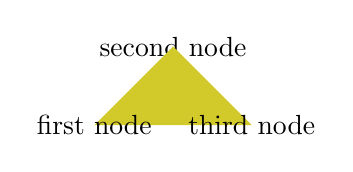
\begin{tikzpicture}[scale = 1]
            \fill [fill=yellow!80!black]
                    (0,0) node  {first node}
                --  (1,1) node[behind path]  {second node}
                --  (2,0) node  {third node};
        \end{tikzpicture}
    \end{minipage}
    \begin{minipage}{0.55\linewidth}
        \begin{lstlisting}[style = latex-side]
    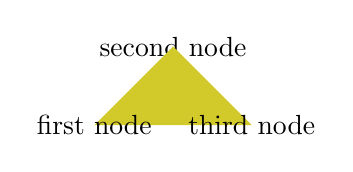
\begin{tikzpicture}[scale = 1]
        \fill [fill=yellow!80!black]
                (0,0) node  {first node}
            --  (1,1) node[behind path]  {second node}
            --  (2,0) node  {third node};
    \end{tikzpicture}
        \end{lstlisting}
    \end{minipage}
    \caption{Node 基本用法}
    \label{Node 基本用法}
\end{figure}

\subsubsection{Node 命令的语法}

\noindent 在 path 中添加 node 的完整语法如下:

\begin{lstlisting}[style = latex]
    \path … node <foreach statements> [<options>] (<name>) at(<coordinate>) :(animation attribute)={<options>} {<node contents>} …;
\end{lstlisting}

\noindent 另一种轻量化的写法

\begin{lstlisting}[style = latex]
    \node [<options>]  (<name>) at(<coordinate>) :(animation);
\end{lstlisting}


\noindent\textbf{主要用法} 
\begin{lstlisting}[style = latex]
    ... node [options] {text} ...;
\end{lstlisting}

\noindent 在 {text} 中添加 node 要显示的文字,[options] 指定样式,下面整理常用 [options]。

\begin{itemize}
    \item 文字与颜色 \\
    除了在 {text} 中指明颜色,在 [options] 也可以使用 [node contents=<text>] 指定文字,且在 [options] 中说明的颜色默认为文字颜色。
    \begin{figure}[H]
        \centering
        \begin{minipage}{0.35\linewidth}
            \centering
            \begin{tikzpicture}[scale = 1]
                \path   (0,0)   node    [blue]  {A}
                        (1,0)   node    [red]   {B}
                        (2,0)   node    [green,node contents=C]
                        (3,0)   node    [node contents=D];
            \end{tikzpicture}
        \end{minipage}
        \begin{minipage}{0.55\linewidth}
            \begin{lstlisting}[style = latex-side]
    \begin{tikzpicture}[scale = 1]
        \path   (0,0)   node    [blue]  {A}
                (1,0)   node    [red]   {B}
                (2,0)   node    [green,node contents=C]
                (3,0)   node    [node contents=D];
    \end{tikzpicture}
            \end{lstlisting}
        \end{minipage}
        \caption{Node 的文字与颜色}
    \end{figure}

    \item 指定位置 \\
    平面位置:[at=<coordinate>]:指定 node 的位置,当 node 在 path 中时,无效。 \\
    图层位置:[behind path]:指定 node 的图层位置,效果见图\ref{Node 基本用法}。默认样式为 [in front of path]

    \item 节点名 \\
    节点名用于后续绘图指定节点,TikZ 允许至多两个节点名。 \\
    节点名:[name=<name>]:节点的名称 \\
    节点别名:[alias=<alias>]:节点别名

    \item 节点形状 \\
    默认节点仅有文字,不具有形状,需要使用 [draw/fill] 命令指定对应形状。\\
    边框:[draw]:显示节点边线;\\
    底色:[fill=<color>]:显示节点底色 \\
    边框形状:[shape = rectangle,circle,ellipse]:shape 可以省略,默认为矩形 rectangle ,更多形状可查阅官方资料。\\
    边框圆角:[rounded corners] \\
    边线数量:[double] \\

    \begin{figure}[H]
        \centering
        \begin{minipage}{0.35\linewidth}
            \centering
            \begin{tikzpicture}[scale = 1]
                \fill[fill=yellow!60!black]
                        (0,0) node [draw, rounded corners] {first node}
                    --  (1,1) node [draw, double, ellipse, behind path] {second node}
                    --  (0,2) node [circle,fill=red!20] {third node};
            \end{tikzpicture}
        \end{minipage}
        \begin{minipage}{0.55\linewidth}
            \begin{lstlisting}[style = latex-side]
    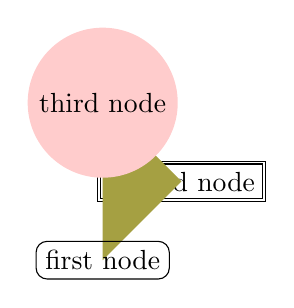
\begin{tikzpicture}[scale = 1]
        \fill[fill=yellow!60!black]
                (0,0) node [draw, rounded corners] {first node}
            --  (1,1) node [draw, double, behind path] {second node}
            --  (0,2) node [circle,fill=red!20] {third node};
    \end{tikzpicture}
            \end{lstlisting}
        \end{minipage}
        \caption{Node 形状}
    \end{figure}

    \item 节点全局样式 \\
    可以通过在 tikzpicture 环境开始处添加说明,给予全局节点样式。\\
    全部样式:[every node/.style = \{\}]\\
    \begin{figure}[H]
        \centering
        \begin{minipage}{0.35\linewidth}
            \centering
            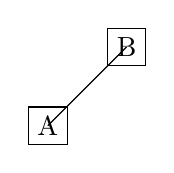
\begin{tikzpicture}[every node/.style={draw}]
                \draw (0,0) node {A} -- (1,1) node {B};
            \end{tikzpicture}
        \end{minipage}
        \begin{minipage}{0.55\linewidth}
            \begin{lstlisting}[style = latex-side]
    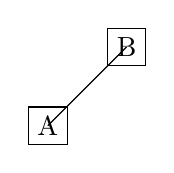
\begin{tikzpicture}[every node/.style={draw}]
        \draw (0,0) node {A} -- (1,1) node {B};
    \end{tikzpicture}
            \end{lstlisting}
        \end{minipage}
        \caption{Node 全部样式}
    \end{figure}
    指定样式:[every <shape> node/.style = \{\}]\\
    \begin{figure}[H]
        \centering
        \begin{minipage}{0.35\linewidth}
            \centering
            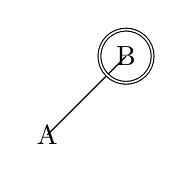
\begin{tikzpicture}[every circle node/.style={draw,double}]
                \draw   (0,0)   node    {A} 
                    --  (1,1)   [circle] node {B};
            \end{tikzpicture}
        \end{minipage}
        \begin{minipage}{0.55\linewidth}
            \begin{lstlisting}[style = latex-side]
    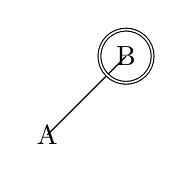
\begin{tikzpicture}[every circle node/.style={draw,double}]
        \draw   (0,0)   node    {A} 
            --  (1,1)   [circle] node {B};
    \end{tikzpicture}
            \end{lstlisting}
        \end{minipage}
        \caption{Node 指定样式}
    \end{figure}
    文字前后缀:[execute at begin/end node = \{text\}] \\
    \begin{figure}[H]
        \centering
        \begin{minipage}{0.35\linewidth}
            \centering
            \begin{tikzpicture}[execute at begin node = {第}, execute at end node = {题}]
                \node [execute at end node = {:}] {一};
            \end{tikzpicture}
        \end{minipage}
        \begin{minipage}{0.55\linewidth}
            \begin{lstlisting}[style = latex-side]
    \begin{tikzpicture}[execute at begin node = {第}, execute at end node = {题}]
        \node [execute at end node = {:}] {一};
    \end{tikzpicture}
            \end{lstlisting}
        \end{minipage}
        \caption{}
    \end{figure}

    \item 其他样式 \\
    填充:[fill = <color>]:填充背景色 \\
    缩放:[scale = <dimension>]:节点缩放 \\
    边框粗细:[linewidth = <dimension>]:边框粗细 \\

\end{itemize}

\noindent\textbf{其他用法} 
\begin{itemize}
    \item 节点动画 \\
    \noindent 通过 :<animation attribute>={<options>},可以设定动画\footnote{部分图形驱动并不支持动画,比如我的也不支持},下面只做简单举例 \\
    \begin{figure}[H]
        \centering
        \begin{minipage}{0.35\linewidth}
            \centering
            \begin{tikzpicture}[scale = 1]
                \node   :fill opacity={0s="1",2s="0",begin on=click}
                        :rotate = {0s="0",2s="90",begin on=click}
                        [fill = blue!20, draw = blue, ultra thick, circle]
                        {click me};
            \end{tikzpicture}
        \end{minipage}
        \begin{minipage}{0.55\linewidth}
            \begin{lstlisting}[style = latex-side]
        \begin{tikzpicture}[scale = 1]
            \node   :fill opacity={0s="1",2s="0",begin on=click}
                    :rotate = {0s="0",2s="90",begin on=click}
                    [fill = blue!20, draw = blue, ultra thick, circle]
                    {click me};
        \end{tikzpicture}
            \end{lstlisting}
        \end{minipage}
        \caption{Node 动画}
    \end{figure}

    \item foreach \\
    foreach 语句仅允许紧跟在 node 之后出现。\\
    语法形式:foreach \textbackslash x in \{\}\\
    在集合{}中可以使用 ... 表示省略类似的内容。\\


    \begin{figure}[H]
        \centering
        \begin{minipage}{0.35\linewidth}
            \centering
            \begin{tikzpicture}[scale = 1]
                \draw (0,0) node foreach \x in {1,2,3} at (\x,0) {\x};
            \end{tikzpicture}
        \end{minipage}
        \begin{minipage}{0.55\linewidth}
            \begin{lstlisting}[style = latex-side]
    % 以下两句效果相同
    \draw (0,0) node foreach \x in {1,2,3} at (\x,0) {\x};
    \tikz \draw (0,0) node at (1,0) {1} node at (2,0) {2} node at (3,0) {3};
            \end{lstlisting}
        \end{minipage}
        \caption{Node 一次迭代}
    \end{figure}

    \begin{figure}[H]
        \centering
        \begin{minipage}{0.35\linewidth}
            \centering
            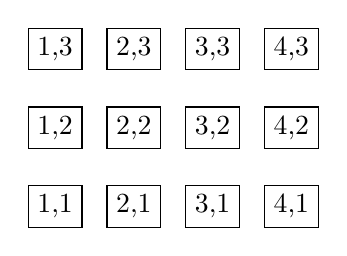
\begin{tikzpicture}[scale = 1]
                \node foreach \x in {1,...,4} foreach \y in {1,2,3} [draw] at (\x,\y) {\x,\y};
            \end{tikzpicture}
        \end{minipage}
        \begin{minipage}{0.55\linewidth}
            \begin{lstlisting}[style = latex-side]
    \node foreach \x in {1,...,4} foreach \y in {1,2,3} [draw] at (\x,\y) {\x,\y};
            \end{lstlisting}
        \end{minipage}
        \caption{Node 两次迭代}
    \end{figure}

    \item scope \\
    scope 用于限定范围,类似高级语言中的命名空间。\\
    和 \LaTeX 中的环境十分相似,scope需要 \textbackslash begin 和 \textbackslash end 来限定范围。\\
    在 \textbackslash begin\{scope\}[name prefix = <text>] 限定范围名。\\
    使用时 "name"+"node name" 即可。\\
    类似的,也可以使用 suffix。 \\
    \begin{figure}[H]
        \centering
        \begin{minipage}{0.35\linewidth}
            \centering
            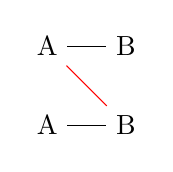
\begin{tikzpicture}[scale = 1]
                \begin{scope}[name prefix = top-]
                    \node (A) at (0,1) {A};
                    \node (B) at (1,1) {B};
                    \draw (A) -- (B);
                \end{scope}
                \begin{scope}[name prefix = buttom-]
                    \node (A) at (0,0) {A};
                    \node (B) at (1,0) {B};
                    \draw (A) -- (B);
                \end{scope}
                \draw [red] (top-A) -- (buttom-B);
            \end{tikzpicture}
        \end{minipage}
        \begin{minipage}{0.55\linewidth}
            \begin{lstlisting}[style = latex-side]
    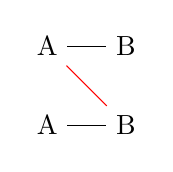
\begin{tikzpicture}[scale = 1]
        \begin{scope}[name prefix = top-]
            \node (A) at (0,1) {A};
            \node (B) at (1,1) {B};
            \draw (A) -- (B);
        \end{scope}
        \begin{scope}[name prefix = buttom-]
            \node (A) at (0,0) {A};
            \node (B) at (1,0) {B};
            \draw (A) -- (B);
        \end{scope}
        \draw [red] (top-A) -- (buttom-B);
    \end{tikzpicture}
            \end{lstlisting}
        \end{minipage}
        \caption{Node:sep}
    \end{figure}
\end{itemize}

\subsubsection{盒模型}

盒模型\footnote{盒模型概念来自css,与这里极其类使,但 TikZ 官方并没有指定这一系列样式的名称},这里指 Node 周围边距,底色等样式的控制。由于比一般的样式控制命令更多,而且重要,单独开一节做笔记。

\begin{itemize}
    \item 边距 sep \hfill(默认: 0.3333em) \\
    总内边距:[inner sep = <dimension>]:边框与内部文字的边距
    \begin{figure}[H]
        \centering
        \begin{minipage}{0.35\linewidth}
            \centering
            \begin{tikzpicture}[scale = 1]
                \draw   (0,0) node [inner sep = 0pt,draw] {0pt}
                        (0,2em) node [inner sep = 5pt,draw] {5pt}
                        (0,4em) node [draw]  {默认};
            \end{tikzpicture}
        \end{minipage}
        \begin{minipage}{0.55\linewidth}
            \begin{lstlisting}[style = latex-side]
    \begin{tikzpicture}[scale = 1]
        \draw   (0,0) node [inner sep = 0pt,draw] {0pt}
                (0,2em) node [inner sep = 5pt,draw] {5pt}
                (0,4em) node [draw]  {默认};
    \end{tikzpicture}
            \end{lstlisting}
        \end{minipage}
        \caption{Node:inner sep}
    \end{figure}

    左右/上下边距:[inner xsep/ysep = <dimension>]\\
    外边距:[outer sep = <dimension>],外边距可能出现一些不准确的问题,可以在环境中加入 [outer sep = auto] 解决,与 inner sep 类使的,也可以指明 x/y 方向外边距。

    \item 最小高度/宽度 \\
    最小高度/宽度用于限制节点与边线的最小距离 \\
    最小距离:[minimum size]:最小高度与宽度 \\
    最小高度:[minimum height], 最小宽度:[minimum width]
    \begin{figure}[H]
        \centering
        \begin{minipage}{0.35\linewidth}
            \centering
            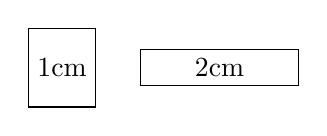
\begin{tikzpicture}[scale = 1]
                \draw   (0,0)   node    [minimum height = 1cm,draw] {1cm}
                        (2,0)   node    [minimum width = 2cm,draw] {2cm};
            \end{tikzpicture}
        \end{minipage}
        \begin{minipage}{0.55\linewidth}
            \begin{lstlisting}[style = latex-side]
    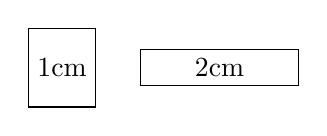
\begin{tikzpicture}[scale = 1]
        \draw   (0,0)   node    [minimum height = 1cm,draw] {1cm}
                (2,0)   node    [minimum width = 2cm,draw] {2cm};
    \end{tikzpicture}
            \end{lstlisting}
        \end{minipage}
        \caption{Node:最小高度/宽度}
    \end{figure}
\end{itemize}

\subsubsection{边框形状}
这里主要备注边框形状相关的内容。
\begin{itemize}
    \item 横纵比 \\
    横纵比:[shape aspect=<aspect ratio>]:外边框形状进行压缩。
    \begin{figure}[H]
        \centering
        \begin{minipage}{0.35\linewidth}
            \centering
            \begin{tikzpicture}[scale = 1]
                \draw   (0,0)   node    [shape aspect=1,diamond,draw] {aspect 1};
                \draw   (0,-2)  node    [shape aspect=2,diamond,draw] {aspect 2};
            \end{tikzpicture}
        \end{minipage}
        \begin{minipage}{0.55\linewidth}
            \begin{lstlisting}[style = latex-side]
    \begin{tikzpicture}[scale = 1]
        \draw   (0,0)   node    [shape aspect=1,diamond,draw] {aspect 1};
        \draw   (0,-2)  node    [shape aspect=2,diamond,draw] {aspect 2};
    \end{tikzpicture}
            \end{lstlisting}
        \end{minipage}
        \caption{Node:aspect}
    \end{figure}

    \item 边框距 \hfill (默认: 1pt)\\
    TikZ 的边框距有两种计算方式,可以使用 [shape border uses incircle = <boolean>] 启动第二种边距计算,效果见下图:
    \begin{figure}[H]
        \centering
        \begin{minipage}{0.35\linewidth}
            \centering
            \begin{tikzpicture}[every node/.style = {isosceles triangle,draw}]
                \node at (0,0) {abc};
                \node [shape border uses incircle] at (2,0) {abc};
                \node [circle,minimum size = 2em] at (0,0) {}; 
                \node [circle,minimum size = 2em] at (2,0) {}; 
            \end{tikzpicture}
        \end{minipage}
        \begin{minipage}{0.55\linewidth}
            \begin{lstlisting}[style = latex-side]
        
            \end{lstlisting}
        \end{minipage}
        \caption{Node:边距}
    \end{figure}

    \item 旋转 \\
    文字旋转:[rotate = <angle>]:文字和边框都将出现旋转。\\
    边框旋转:[rotate = <angle>]:仅边框旋转。 \\
    \begin{figure}[H]
        \centering
        \begin{minipage}{0.35\linewidth}
            \centering
            \begin{tikzpicture}[every node/.style={shape=trapezium, draw, shape border uses incircle}]
                \node at (0,0) (A) {A};
                \node [shape border rotate=30] at (1.5,0) {B};
                \node [rotate=30] at (3,0) {C};
            \end{tikzpicture}
        \end{minipage}
        \begin{minipage}{0.55\linewidth}
            \begin{lstlisting}[style = latex-side]
    \begin{tikzpicture}[every node/.style={shape=trapezium, draw, shape border usincircle}]
        \node at (0,0) (A) {A};
        \node [shape border rotate=30] at (1.5,0) {B};
        \node [rotate=30] at (3,0) {C};
    \end{tikzpicture}
            \end{lstlisting}
        \end{minipage}
        \caption{Node:旋转}
    \end{figure}

    \item 边框粗细 \\
    粗细:[linewidth = <dimension>]
    \begin{figure}[H]
        \centering
        \begin{minipage}{0.35\linewidth}
            \centering
            
\begin{tikzpicture}[scale = 1]
                \node [line width=2,draw] at (0,0) {A};
            \end{tikzpicture}
        \end{minipage}
        \begin{minipage}{0.55\linewidth}
            \begin{lstlisting}[style = latex-side]
    
\begin{tikzpicture}[scale = 1]
        \node [line width=2,draw] at (0,0) {A};
    \end{tikzpicture}
            \end{lstlisting}
        \end{minipage}
        \caption{Node:边框粗细}
    \end{figure}
\end{itemize}

\subsection{节点样式}
\subsubsection{分割节点}
在 node 文字{}中使用 \verb|\|nodepart[<options>]\{<part name>\} 可以对节点进行切割;注意此时的 shape 形状后需加上 split,否则无效。同时需要声明 \verb|\|use tikzlibrary {shapes.multipart}

\begin{figure}[H]
    \centering
    \begin{minipage}{0.35\linewidth}
        \centering
        \begin{tikzpicture}[scale = 1]
            \node [circle split,draw,double] {$q_1$ \nodepart{lower} $00$};
        \end{tikzpicture}
    \end{minipage}
    \begin{minipage}{0.55\linewidth}
        \begin{lstlisting}[style = latex-side]
    \begin{tikzpicture}[scale = 1]
        \node [circle split,draw,double] {$q_1$ \nodepart{lower} $00$};
    \end{tikzpicture}
        \end{lstlisting}
    \end{minipage}
    \caption{Node:分割节点}
\end{figure}

对于批量修改节点样式,可以使用类似 every lower node part/.style = color 的方法。

\begin{figure}[H]
    \centering
    \begin{minipage}{0.35\linewidth}
        \centering
        \begin{tikzpicture}[every lower node part/.style = red]
            \node [circle split,draw] {$q_1$ \nodepart{lower} $00$};
        \end{tikzpicture}
    \end{minipage}
    \begin{minipage}{0.55\linewidth}
        \begin{lstlisting}[style = latex-side]
    \begin{tikzpicture}[every lower node part/.style = red]
        \node [circle split,draw] {$q_1$ \nodepart{lower} $00$};
    \end{tikzpicture}
        \end{lstlisting}
    \end{minipage}
    \caption{Node:分割节点样式}
\end{figure}

\subsubsection{节点文字}

文字本身包含颜色,字体,大小等样式,具体控制如下:
\begin{itemize}
    \item 颜色 \\
    文字颜色:[color = <color>],这里的color可以省略,注意在节点中的颜色属性只影响节点文字,这与 \verb|\|draw 不同

    \begin{figure}[H]
        \centering
        \begin{minipage}{0.35\linewidth}
            \centering
            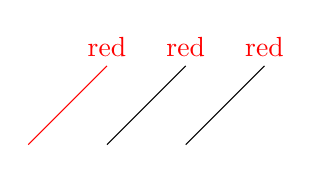
\begin{tikzpicture}[scale = 1]
                \draw[red]          (0,0) -- +(1,1) node[above] {red};
                \draw[text = red]   (1,0) -- +(1,1) node[above] {red};
                \draw               (2,0) -- +(1,1) node[above,red] {red};
            \end{tikzpicture}
        \end{minipage}
        \begin{minipage}{0.55\linewidth}
            \begin{lstlisting}[style = latex-side]
    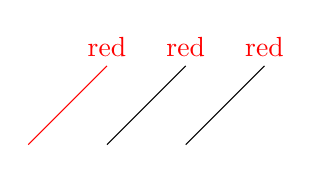
\begin{tikzpicture}[scale = 1]
        \draw[red]          (0,0) -- +(1,1) node[above] {red};
        \draw[text = red]   (1,0) -- +(1,1) node[above] {red};
        \draw               (2,0) -- +(1,1) node[above,red] {red};
    \end{tikzpicture}
            \end{lstlisting}
        \end{minipage}
        \caption{Node:文字颜色}
    \end{figure}

    \item 不透明度 \\
    不透明度:[opacity = <value>],注意这里是不透明度,1表示完全不透明。

    \begin{figure}[H]
        \centering
        \begin{minipage}{0.35\linewidth}
            \centering
            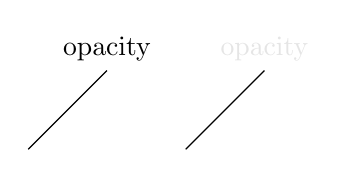
\begin{tikzpicture}[scale = 1]
                \draw[opacity = 1]          (0,0) -- +(1,1) node[above] {opacity};
                \draw               (2,0) -- +(1,1) node[above,opacity = 0.1] {opacity};
            \end{tikzpicture}
        \end{minipage}
        \begin{minipage}{0.55\linewidth}
            \begin{lstlisting}[style = latex-side]
    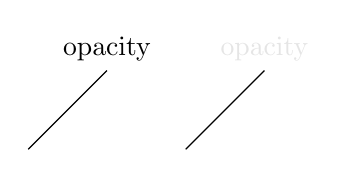
\begin{tikzpicture}[scale = 1]
        \draw[opacity = 1]          (0,0) -- +(1,1) node[above] {opacity};
        \draw               (2,0) -- +(1,1) node[above,opacity = 0.1] {opacity};
    \end{tikzpicture}
            \end{lstlisting}
        \end{minipage}
        \caption{Node:文字透明度}
    \end{figure}

    \item 文字字体 \\
    文字字体:[node font = <font commands>],这里的 node 可以省略。注意这里的 font 既可以指字体族,也可以控制字体大小。

    \begin{figure}[H]
        \centering
        \begin{minipage}{0.35\linewidth}
            \centering
            \begin{tikzpicture}[every text node part/.style={font=\itshape},every lower node part/.style={font=\footnotesize}]
                \draw[node font=\itshape] (1,0) -- +(1,1) node[above] {italic};
                \draw[node font=\tiny] (2,0) -- +(1,1) node[above] {tiny};
                \node [circle split,draw] at (4,0) {state \nodepart{lower} output};
            \end{tikzpicture}
        \end{minipage}
        \begin{minipage}{0.55\linewidth}
            \begin{lstlisting}[style = latex-side]
    \begin{tikzpicture}[every text node part/.style={font=\itshape},every lower node part/.style={font=\footnotesize}]
        \draw[node font=\itshape] (1,0) -- +(1,1) node[above] {italic};
        \draw[node font=\tiny] (2,0) -- +(1,1) node[above] {tiny};
        \node [circle split,draw] at (4,0) {state \nodepart{lower} output};
    \end{tikzpicture}
            \end{lstlisting}
        \end{minipage}
        \caption{Node:文字字体}
    \end{figure}

    \item 文字高度与深度 \\
    文字高度:[text height = <dimension>] \\
    文字深度:[text depth = <dimension>] \\
    这两个属性并不常用,一般情况下尽量用 inner sep 代替。
\end{itemize}

\subsubsection{节点文本}

文本格式包括文本框的长宽,对齐方式等。

\begin{itemize}
    \item 节点文本框\\
    与正文中的文本类似,节点中的文本也可以实现公式,换行,表格等功能。

    \begin{figure}[H]
        \centering
        \begin{minipage}{0.35\linewidth}
            \centering
            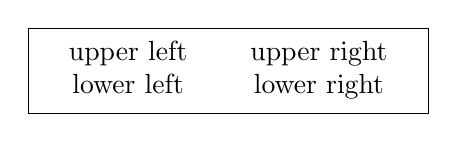
\begin{tikzpicture}[scale = 1]
                \node [draw] {
                    \begin{tabular}{cc}
                        upper left & upper right\\
                        lower left & lower right
                    \end{tabular}
                };
            \end{tikzpicture}
        \end{minipage}
        \begin{minipage}{0.55\linewidth}
            \begin{lstlisting}[style = latex-side]
    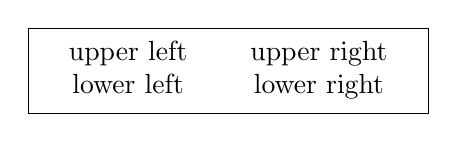
\begin{tikzpicture}[scale = 1]
        \node [draw] {
            \begin{tabular}{cc}
                upper left & upper right\\
                lower left & lower right
            \end{tabular}
        };
    \end{tikzpicture}
            \end{lstlisting}
        \end{minipage}
        \caption{Node:节点文本框}
    \end{figure}

    \item 文本对齐\\
    对齐:[align = <alignment option>],设置对其方式。

    \begin{figure}[H]
        \centering
        \begin{minipage}{0.35\linewidth}
            \centering
            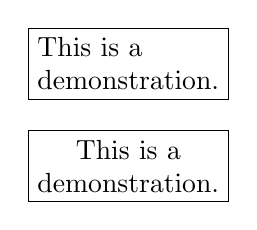
\begin{tikzpicture}[scale = 1]
                \node[draw,align=left]at (0,0) {This is a\\demonstration.};
                \node[draw,align=center] at (0,-1.3) {This is a\\demonstration.};
            \end{tikzpicture}
        \end{minipage}
        \begin{minipage}{0.55\linewidth}
            \begin{lstlisting}[style = latex-side]
    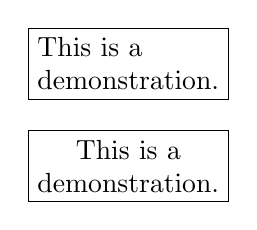
\begin{tikzpicture}[scale = 1]
        \node[draw,align=left]at (0,0) {This is a\\demonstration.};
        \node[draw,align=center] at (0,-1.3) {This is a\\demonstration.};
    \end{tikzpicture}
            \end{lstlisting}
        \end{minipage}
        \caption{Node:文本对齐}
    \end{figure}

    \noindent 文本对齐会自动分割长单词,可以使用 align = flush <alignment option> 来取消长单词。
    \begin{figure}[H]
        \centering
        \begin{minipage}{0.35\linewidth}
            \centering
            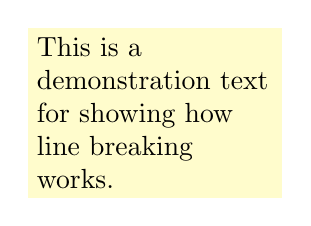
\begin{tikzpicture}[scale = 1]
                \node[fill=yellow!20,text width=3cm,align=flush left] {This is a demonstration text for showing how line breaking works.};
            \end{tikzpicture}
        \end{minipage}
        \begin{minipage}{0.55\linewidth}
            \begin{lstlisting}[style = latex-side]
    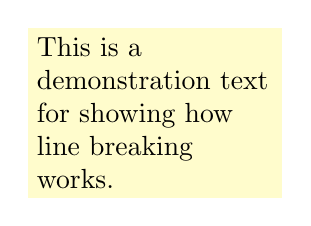
\begin{tikzpicture}[scale = 1]
        \node[fill=yellow!20,text width=3cm,align=flush left] {This is a demonstration text for showing how line breaking works.};
    \end{tikzpicture}
            \end{lstlisting}
        \end{minipage}
        \caption{Node:分割长单词}
    \end{figure}

    alignment option 具体参数见属性百科:

    \item 文本宽度 \\
    文本宽:[text width = <dimension>]:限定最大文本宽

    \begin{figure}[H]
        \centering
        \begin{minipage}{0.35\linewidth}
            \centering
            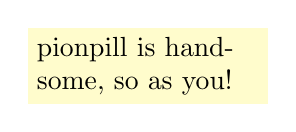
\begin{tikzpicture}[scale = 1]
                \draw (0,0) node [text width=8em, fill = yellow!20] {pionpill is handsome, so as you!};
            \end{tikzpicture}
        \end{minipage}
        \begin{minipage}{0.55\linewidth}
            \begin{lstlisting}[style = latex-side]
    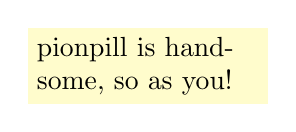
\begin{tikzpicture}[scale = 1]
        \draw (0,0) node [text width=8em, fill = yellow!20] {pionpill is handsome, so as you!};
    \end{tikzpicture}
            \end{lstlisting}
        \end{minipage}
        \caption{Node:文本宽度}
    \end{figure}
\end{itemize}

\subsubsection{节点变换}
常用的节点的变换(transform)修饰有缩放与旋转。

\begin{figure}[H]
    \centering
    \begin{minipage}{0.35\linewidth}
        \centering
        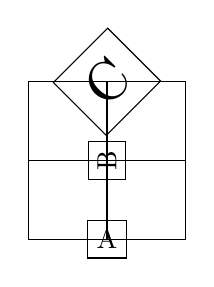
\begin{tikzpicture}[every node/.style = draw]
            \draw (0,0) grid (2,2);
            \draw (1,0) node {A};
            \draw (1,1) node [rotate = 90] {B};
            \draw (1,2) node [rotate = 45,scale = 2] {C};
        \end{tikzpicture}
    \end{minipage}
    \begin{minipage}{0.55\linewidth}
        \begin{lstlisting}[style = latex-side]
    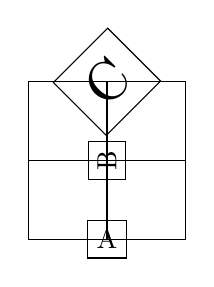
\begin{tikzpicture}[every node/.style = draw]
        \draw (0,0) grid (2,2);
        \draw (1,0) node {A};
        \draw (1,1) node [rotate = 90] {B};
        \draw (1,2) node [rotate = 45,scale = 2] {C};
    \end{tikzpicture}
        \end{lstlisting}
    \end{minipage}
    \caption{Node:节点变换}
\end{figure}

\subsubsection{节点复用}

节点复用,即在使用过节点后,再使用节点。使用 also 关键字,即可启用之前定义过的节点。复用的节点无法添加文字。

\begin{figure}[H]
    \centering
    \begin{minipage}{0.35\linewidth}
        \centering
        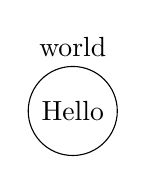
\begin{tikzpicture}[scale = 1]
            \node [circle,draw] (a) {Hello};
            \node also [label=above:world] (a);
        \end{tikzpicture}
    \end{minipage}
    \begin{minipage}{0.55\linewidth}
        \begin{lstlisting}[style = latex-side]
    \begin{tikzpicture}[scale = 1]
        \node [circle,draw] (a) {Hello};
        \node also [label=above:world] (a);
    \end{tikzpicture}
        \end{lstlisting}
    \end{minipage}
    \caption{Node:also}
\end{figure}

类似的,也可以使用 [late options = \{\}] 达到同样的效果。

\begin{figure}[H]
    \centering
    \begin{minipage}{0.35\linewidth}
        \centering
        \begin{tikzpicture}[scale = 1]
            \node [draw,circle] (a) {Hello};
            \path [late options = {name=a,label=above:world}];
        \end{tikzpicture}
    \end{minipage}
    \begin{minipage}{0.55\linewidth}
        \begin{lstlisting}[style = latex-side]
    \begin{tikzpicture}[scale = 1]
        \node [draw,circle] (a) {Hello};
        \path [late options = {name=a,label=above:world}];
    \end{tikzpicture}
        \end{lstlisting}
    \end{minipage}
    \caption{Node:late option}
\end{figure}

\subsection{节点布局}
\subsubsection{定位}

节点的位置往往由与之相关的坐标决定,默认以坐标为中心生成节点,同时也可在坐标周围生成节点。

\begin{itemize}
    \item 节点锚点 \\
    锚点:[anchor = <anchor name>]:锚点属性决定了节点将在坐标的哪个方向生成。\\
    这里 anchor 的意思是坐标位于节点的方向。
    \begin{figure}[H]
        \centering
        \begin{minipage}{0.35\linewidth}
            \centering
            \begin{tikzpicture}[scale = 1]
                \draw (0,0) node [anchor = north] {north};
                \draw (1,1) node [anchor = south west] {south west};
                \draw (0,0) rectangle (1,1);
            \end{tikzpicture}
        \end{minipage}
        \begin{minipage}{0.55\linewidth}
            \begin{lstlisting}[style = latex-side]
        
            \end{lstlisting}
        \end{minipage}
        \caption{Node:锚点}
    \end{figure}

    \item 偏移 \\
    偏移:[<offset>]:无需属性名,效果与 anchor 类似,但是能更精确地控制偏移量。

    \begin{figure}[H]
        \centering
        \begin{minipage}{0.35\linewidth}
            \centering
            \begin{tikzpicture}[scale = 1]
                \fill (0,0) circle (2pt) node [above] {above};
                \fill (0,-1) circle (2pt) node [above=5pt] {above};
            \end{tikzpicture}
        \end{minipage}
        \begin{minipage}{0.55\linewidth}
            \begin{lstlisting}[style = latex-side]
    \begin{tikzpicture}[scale = 1]
        \fill (0,0) circle (2pt) node [above] {above};
        \fill (0,-1) circle (2pt) node [above=5pt] {above};
    \end{tikzpicture}
            \end{lstlisting}
        \end{minipage}
        \caption{Node:偏移}
    \end{figure}
\end{itemize}

\subsubsection{高阶布局}

除了简单的定位,还可以使用 positioning 包来进行更为高阶的定位操作。在启动了该包后,原本的 <dimension> 参数将被提升为 <specification>。<specification> 参数通常由两部分组成:<shifting part> + <of-part>

<shifting part> 为主要控制参数,通常有三种形式:

\begin{itemize}
    \item <dimension> 形式 \\
    这种形式在 <dimension> 参数的基础上,还可以使用数学式。

    \begin{figure}[H]
        \centering
        \begin{minipage}{0.35\linewidth}
            \centering
            \begin{tikzpicture}[scale = 1]
                \draw (0,0) grid (2,2);
                \node at (1,1) [above = 2pt+3pt,fill=white] {above};
            \end{tikzpicture}
        \end{minipage}
        \begin{minipage}{0.55\linewidth}
            \begin{lstlisting}[style = latex-side]
    \begin{tikzpicture}[scale = 1]
        \draw (0,0) grid (2,2);
        \node at (1,1) [above = 2pt+3pt,fill=white] {above};
    \end{tikzpicture}
            \end{lstlisting}
        \end{minipage}
        \caption{Node:高阶布局-数学形式}
    \end{figure}

    \item <number> 形式 \\
    这种形式可以不包含单位,其他和上面那个差别不大。
    
    \begin{figure}[H]
        \centering
        \begin{minipage}{0.35\linewidth}
            \centering
            \begin{tikzpicture}[scale = 1]
                \draw (0,0) grid (2,2);
                \node at (1,1) [above = .2,fill=white] {above};  
            \end{tikzpicture}
        \end{minipage}
        \begin{minipage}{0.55\linewidth}
            \begin{lstlisting}[style = latex-side]
    \begin{tikzpicture}[scale = 1]
        \draw (0,0) grid (2,2);
        \node at (1,1) [above = .2,fill=white] {above};  
        % south border of the node is now 2mm above (1,1)
    \end{tikzpicture}
            \end{lstlisting}
        \end{minipage}
        \caption{Node:高阶布局-数字形式}
    \end{figure}

    \item and 组合形式 \\
    可以通过 and 将多个偏移修饰组合,这里 and 的作用并不明显,下一节将详细说明。

    \begin{figure}[H]
        \centering
        \begin{minipage}{0.35\linewidth}
            \centering
            \begin{tikzpicture}[scale = 1]
                \draw (0,0) grid (2,2);
                \node at (1,1) [above = .2 and 2mm,fill=white] {above};  
            \end{tikzpicture}
        \end{minipage}
        \begin{minipage}{0.55\linewidth}
            \begin{lstlisting}[style = latex-side]
    \begin{tikzpicture}[scale = 1]
        \draw (0,0) grid (2,2);
        \node at (1,1) [above = .2 and 2mm,fill=white] {above};  
        % south border of the node is also 2mm above (1,1)
    \end{tikzpicture}
            \end{lstlisting}
        \end{minipage}
        \caption{Node:高阶布局-组合形式}
    \end{figure}
\end{itemize}

<of-part> 可以进行相对定位,注意点如下:

\begin{itemize}
    \item 以坐标为参照的定位 \\
    通过 of 关键字可以调用坐标点的方位进行相对定位。

    \begin{figure}[H]
        \centering
        \begin{minipage}{0.35\linewidth}
            \centering
            \begin{tikzpicture}[scale = 1]
                \draw (0,0) grid (2,2);
                \node (point) [draw] at (1,1) {point};
                \node [above = 5mm of point.north east,draw] {north east};
            \end{tikzpicture}
        \end{minipage}
        \begin{minipage}{0.55\linewidth}
            \begin{lstlisting}[style = latex-side]
    \begin{tikzpicture}[scale = 1]
        \draw (0,0) grid (2,2);
        \node (point) [draw] at (1,1) {point};
        \node [above = 5mm of point.north east,draw] {north east};
    \end{tikzpicture}
            \end{lstlisting}
        \end{minipage}
        \caption{Node:of-part 坐标定位}
    \end{figure}

    定位逻辑:首先找到 point 的 north east 位置,然后向 above 方向移动了 5mm。\\
    不止于坐标,一般别名都可以作为定位对象。

    \item 距离测算 \\
    默认状态下的偏移距离为边界之间的距离,而不是中心距。

    \begin{figure}[H]
        \centering
        \begin{minipage}{0.35\linewidth}
            \centering
            \begin{tikzpicture}[every node/.style = draw]
                \draw (0,0) grid (2,2);
                \node (point1) at (1,1) {point1};
                \node (point2) [above = 1cm of point1] {point2};
                \node (point3) [below = 1cm of point1.center] {point3};
            \end{tikzpicture}
        \end{minipage}
        \begin{minipage}{0.55\linewidth}
            \begin{lstlisting}[style = latex-side]
    \begin{tikzpicture}[every node/.style = draw]
        \draw (0,0) grid (2,2);
        \node (point1) at (1,1) {point1};
        \node (point2) [above = 1cm of point1] {point2};
        \node (point3) [below = 1cm of point1.center] {point3};
    \end{tikzpicture}
            \end{lstlisting}
        \end{minipage}
        \caption{Node:距离测算}
    \end{figure}

    发现没什么好办法获得中心距。

    \item 网格距 \\
    网格距使用 on grid 将全部距离都定位在网格上,以获得中心距。

    \begin{figure}[H]
        \centering
        \begin{minipage}{0.35\linewidth}
            \centering
            \begin{tikzpicture}[every node/.style = draw]
                \draw (0,0) grid (2,3);
                \node (a1) at (0,0) {normal};
                \node (a2) [above = 1 of a1] {1cm};
                \node (a3) [above = 1 of a2] {1cm};
                \begin{scope}[on grid]
                    \node (b1) at (2,0) {grid};
                    \node (b2) [above = 1 of b1] {1cm};
                    \node (b3) [above = 1 of b2] {1cm};
                \end{scope}
            \end{tikzpicture}
        \end{minipage}
        \begin{minipage}{0.55\linewidth}
            \begin{lstlisting}[style = latex-side]
    \begin{tikzpicture}[every node/.style = draw]
        \draw (0,0) grid (2,3);
        \node (a1) at (0,0) {normal};
        \node (a2) [above = 1 of a1] {1cm};
        \node (a3) [above = 1 of a2] {1cm};
        \begin{scope}[on grid]
            \node (b1) at (2,0) {grid};
            \node (b2) [above = 1 of b1] {1cm};
            \node (b3) [above = 1 of b2] {1cm};
        \end{scope}
    \end{tikzpicture}
            \end{lstlisting}
        \end{minipage}
        \caption{Node:on gird}
    \end{figure}
    
    \item and 组合形式 \\
    上文已说过 and 可以添加多个修饰,这里来看一下用不用 and 的区别。
    
    \begin{figure}[H]
        \centering
        \begin{minipage}{0.3\linewidth}
            \centering
            \begin{tikzpicture}[every node/.style = draw]
                \begin{scope}[node distance = 5mm]
                    \node (a) at (2,3) {a};
                    \node [left=of a] {1}; \node [right=of a] {2};
                    \node [above=of a] {3}; \node [below=of a] {4};
                    \node [above left=of a] {5}; \node [above right=of a] {6};
                    \node [below left=of a] {7}; \node [below right=of a] {8};
                \end{scope}
                \begin{scope}[node distance = 5mm and 5mm]
                    \node (a) at (2,0) {a};
                    \node [left=of a] {1}; \node [right=of a] {2};
                    \node [above=of a] {3}; \node [below=of a] {4};
                    \node [above left=of a] {5}; \node [above right=of a] {6};
                    \node [below left=of a] {7}; \node [below right=of a] {8};
                \end{scope}
            \end{tikzpicture}
        \end{minipage}
        \begin{minipage}{0.6\linewidth}
            \begin{lstlisting}[style = latex-side]
    \begin{tikzpicture}[every node/.style = draw]
        \begin{scope}[node distance = 5mm]
            \node (a) at (2,3) {a};
            \node [left=of a] {1}; \node [right=of a] {2};
            \node [above=of a] {3}; \node [below=of a] {4};
            \node [above left=of a] {5}; \node [above right=of a] {6};
            \node [below left=of a] {7}; \node [below right=of a] {8};
        \end{scope}
        \begin{scope}[node distance = 5mm and 5mm]
            \node (a) at (2,0) {a};
            \node [left=of a] {1}; \node [right=of a] {2};
            \node [above=of a] {3}; \node [below=of a] {4};
            \node [above left=of a] {5}; \node [above right=of a] {6};
            \node [below left=of a] {7}; \node [below right=of a] {8};
        \end{scope}
    \end{tikzpicture}
            \end{lstlisting}
        \end{minipage}
        \caption{Node:and 详解}
    \end{figure}
\end{itemize}

\subsubsection{节点集}

使用 fit 修饰可以将指定的节点圈起来。需要使用 fit 包

\begin{figure}[H]
    \centering
    \begin{minipage}{0.35\linewidth}
        \centering
        \begin{tikzpicture}
            \node (a) at (0,0) {a};
            \node (b) at (1,1) {b};
            \node (c) at (0,2) {b};
            \node[draw=red,inner sep=0pt,thick,ellipse,fit=(a) (b) (c)] {};
        \end{tikzpicture}
    \end{minipage}
    \begin{minipage}{0.55\linewidth}
        \begin{lstlisting}[style = latex-side]
    \begin{tikzpicture}
        \node (a) at (0,0) {a};
        \node (b) at (1,1) {b};
        \node (c) at (0,2) {b};
        \node[draw=red,inner sep=0pt,thick,ellipse,fit=(a) (b) (c)] {};
    \end{tikzpicture}
        \end{lstlisting}
    \end{minipage}
    \caption{Node:fit}
\end{figure}

\subsection{节点交互}
\subsubsection{曲线上的节点}

节点交互指节点与其他 TikZ 图形之间的组合,例如在线段上某一位置插入节点。

\begin{itemize}
    \item 节点插入位置\\
    插入位置:[pos = <fraction>],按线段长度比插入到对应的位置。

    \begin{figure}[H]
        \centering
        \begin{minipage}{0.35\linewidth}
            \centering
            \begin{tikzpicture}[scale = 1]
                \draw (0,0)  -- (3,1) node [pos = 0] {0} node [pos = 0.5] {0.5} node [pos = 0.9] {0.9};
            \end{tikzpicture}
        \end{minipage}
        \begin{minipage}{0.55\linewidth}
            \begin{lstlisting}[style = latex-side]
    \begin{tikzpicture}[scale = 1]
        \draw (0,0)  -- (3,1) node [pos = 0] {0} node [pos = 0.5] {0.5} node [pos = 0.9] {0.9};
    \end{tikzpicture}
            \end{lstlisting}
        \end{minipage}
        \caption{Node:节点插入位置}
    \end{figure}

    值得注意的是,pos在曲线中代表的并不是长度比,pos 的具体计算方式比较复杂在这里不做说明。

    \begin{figure}[H]
        \centering
        \begin{minipage}{0.35\linewidth}
            \centering
            \begin{tikzpicture}[scale = 1]
                \draw (0,0) .. controls +(right:3.5cm) and + (right:3.5cm) .. (0,3) node foreach \x in {0,0.125,...,1} [pos = \x,scale =3,radius = 1pt] {.};
                \draw (0,-2) |- (3,-1) node[pos=0]{0} node[pos=0.5]{1/2} node[pos=0.9]{9/10};
            \end{tikzpicture}
        \end{minipage}
        \begin{minipage}{0.55\linewidth}
            \begin{lstlisting}[style = latex-side]
    \begin{tikzpicture}[scale = 1]
        \draw (0,0) .. controls +(right:3.5cm) and + (right:3.5cm) .. (0,3) node foreach \x in {0,0.125,...,1} [pos = \x,scale =3,radius = 1pt] {.};
        \draw (0,-2) |- (3,-1) node[pos=0]{0} node[pos=0.5]{1/2} node[pos=0.9]{9/10};
    \end{tikzpicture}
            \end{lstlisting}
        \end{minipage}
        \caption{Node:pos 位置}
    \end{figure}

    \item 节点自动位置 \\
    自动位置:[auto = <direction>] 这个修饰将节点自动生成在线段的某一方位,如果设置了 auto 的值,则为 auto 方向,如果没有设置,则为最近一个设置的方向,如果设置了 none,则禁用 auto。其具体的规则请查阅TikZ官方文档。

    \begin{figure}[H]
        \centering
        \begin{minipage}{0.35\linewidth}
            \centering
            \begin{tikzpicture}[scale=.8,auto=left,every node/.style={circle,fill=blue!20}]
                \node (a) at (-1,-2) {a};
                \node (b) at ( 1,-2) {b};
                \node (c) at ( 2,-1) {c};
                \node (d) at ( 2, 1) {d};
                \node (e) at ( 1, 2) {e};
                \node (f) at (-1, 2) {f};
                \node (g) at (-2, 1) {g};
                \node (h) at (-2,-1) {h};
                \foreach \from/\to in {a/b,b/c,c/d,d/e,e/f,f/g,g/h,h/a}
                \draw [->] (\from) -- (\to)
                node[midway,fill=red!20] {\from--\to};
            \end{tikzpicture}
        \end{minipage}
        \begin{minipage}{0.55\linewidth}
            \begin{lstlisting}[style = latex-side]
    \begin{tikzpicture}[scale=.8,auto=left,every node/.style={circle,fill=blue!20}]
        \node (a) at (-1,-2) {a};
        \node (b) at ( 1,-2) {b};
        \node (c) at ( 2,-1) {c};
        \node (d) at ( 2, 1) {d};
        \node (e) at ( 1, 2) {e};
        \node (f) at (-1, 2) {f};
        \node (g) at (-2, 1) {g};
        \node (h) at (-2,-1) {h};
        \foreach \from/\to in {a/b,b/c,c/d,d/e,e/f,f/g,g/h,h/a}
        \draw [->] (\from) -- (\to)
        node[midway,fill=red!20] {\from--\to};
    \end{tikzpicture}
            \end{lstlisting}
        \end{minipage}
        \caption{Node:auto}
    \end{figure}

    \item 方位交换 \\
    交换:[swap]:与原方向相反,常常配合 auto 使用。需要用的 automate 包。swap 可以用 ' 来代替。
    \begin{figure}[H]
        \centering
        \begin{minipage}{1\linewidth}
            \centering
            \begin{tikzpicture}[auto]
                \draw (0.5,0) .. controls (9,6) and (-5,6) .. (3.5,0) 
                    node foreach \pos in {0,0.1,0.2,0.3,0.4,0.5,0.6,0.7,0.8,0.9,1} [pos=\pos,swap,fill=red!20] {\pos}
                    node foreach \pos in {0.025,0.2,0.4,0.6,0.8,0.975} [pos=\pos,fill=blue!20] {\pos};
            \end{tikzpicture}
        \end{minipage}
        \begin{minipage}{0.7\linewidth}
            \begin{lstlisting}[style = latex-side]
    \begin{tikzpicture}[auto]
        \draw (0.5,0) .. controls (9,6) and (-5,6) .. (3.5,0) node foreach \pos in {0,0.1,0.2,0.3,0.4,0.5,0.6,0.7,0.8,0.9,1} [pos=\pos,swap,fill=red!20] {\pos} node foreach \pos in {0.025,0.2,0.4,0.6,0.8,0.975} [pos=\pos,fill=blue!20] {\pos};
    \end{tikzpicture}
            \end{lstlisting}
        \end{minipage}
        \caption{Node:swap}
    \end{figure}

    \item 倾斜 \\
    倾斜:[sloped]:倾斜可以让文本和曲线保持统一方向

    \begin{figure}[H]
        \centering
        \begin{minipage}{0.35\linewidth}
            \centering
            \begin{tikzpicture}[scale = 1]
                \draw (0,0) .. controls +(up:2cm) and + (left:2cm) .. (1,3) node foreach \p in {0.1,0.35,0.7,1} [pos = \p,sloped,above] {\p};
            \end{tikzpicture}
        \end{minipage}
        \begin{minipage}{0.55\linewidth}
            \begin{lstlisting}[style = latex-side]
                \begin{tikzpicture}[scale = 1]
                    \draw (0,0) .. controls +(up:2cm) and + (left:2cm) .. (1,3) node foreach \p in {0.1,0.35,0.7,1} [pos = \p,sloped,above] {\p};
                \end{tikzpicture}
            \end{lstlisting}
        \end{minipage}
        \caption{Node:sloped}
    \end{figure}

    \item 颠倒 \\
    颠倒:[allow upside down]:强制节点按指定方向生成,这可能对导致文字出现奇怪的朝向。

    \begin{figure}[H]
        \centering
        \begin{minipage}{0.35\linewidth}
            \centering
            \begin{tikzpicture}[scale = 1]
                \draw (0,0) .. controls +(up:2cm) and + (left:2cm) .. (1,3) node foreach \p in {0.1,0.35,0.7,1} [pos = \p,sloped,above,allow upside down] {\p};
            \end{tikzpicture}
        \end{minipage}
        \begin{minipage}{0.55\linewidth}
            \begin{lstlisting}[style = latex-side]
                \begin{tikzpicture}[scale = 1]
                    \draw (0,0) .. controls +(up:2cm) and + (left:2cm) .. (1,3) node foreach \p in {0.1,0.35,0.7,1} [pos = \p,sloped,above,allow upside down] {\p};
                \end{tikzpicture}
            \end{lstlisting}
        \end{minipage}
        \caption{Node:sloped}
    \end{figure}

    \item 预定义位置\\
    TikZ 预定义了几个 pos 对应的位置,可以直接使用其名称。

    \begin{figure}[H]
        \centering
        \begin{minipage}{0.35\linewidth}
            \centering
            \begin{tikzpicture}[scale = 0.8]
                \draw (0,0) .. controls +(up:2cm) and +(left:3cm) .. (1,5)
                    node[at end] {at end}
                    node[very near end] {very near end}
                    node[near end] {near end}
                    node[midway] {midway}
                    node[near start] {near start}
                    node[very near start] {very near start}
                    node[at start] {at start};
            \end{tikzpicture}
        \end{minipage}
        \begin{minipage}{0.55\linewidth}
            \begin{lstlisting}[style = latex-side]
    \begin{tikzpicture}[scale = 0.8]
        \draw (0,0) .. controls +(up:2cm) and +(left:3cm) .. (1,5)
            node[at end] {at end}
            node[very near end] {very near end}
            node[near end] {near end}
            node[midway] {midway}
            node[near start] {near start}
            node[very near start] {very near start}
            node[at start] {at start};
    \end{tikzpicture}
            \end{lstlisting}
        \end{minipage}
        \caption{Node:预定义位置}
    \end{figure}

    预定义位置具体位置如下表:

    \begin{table}[H]
        \centering
        \caption{Node:预定义位置}
        \label{table:Node:预定义位置}
        \setlength{\tabcolsep}{4mm}
        \begin{tabular}{c|cc|c}
            \toprule
            \textbf{位置} & \textbf{对应pos值} & \textbf{位置} & \textbf{对应pos值} \\
            \midrule
            at start & 0 & very near start & 0.125 \\
            near start & 0.25 & midway & 0.5 \\
            near end & 0.75 & very near end & 0.875 \\
            at end & 1 &  &  \\
            \bottomrule
        \end{tabular}
    \end{table}

\end{itemize}

\subsubsection{节点之间交互}

节点之间除了默认的连线位置外,还可以使用 node.<anchor> 指定连接的位置。此外,与曲线类似,节点之间的连线也有多种样式。

\begin{figure}[H]
    \centering
    \begin{minipage}{0.35\linewidth}
        \centering
        \begin{tikzpicture}[scale = 1]
            \path (0,0) node (x) {Hello!}
                  (3,1) node[circle,draw] (y) {World!};
            \draw [->,blue] (x.center) -- (y);
            \draw [->,red] (x) -| node[near start,below] {label} (y);
            \draw [->,orange] (x) .. controls +(up:1cm) and +(left:1cm) .. node[above,sloped] {label} (y);
        \end{tikzpicture}
    \end{minipage}
    \begin{minipage}{0.55\linewidth}
        \begin{lstlisting}[style = latex-side]
    \begin{tikzpicture}[scale = 1]
        \path (0,0) node (x) {Hello!}
              (3,1) node[circle,draw] (y) {World!};
        \draw [->,blue] (x.center) -- (y);
        \draw [->,red] (x) -| node[near start,below] {label} (y);
        \draw [->,orange] (x) .. controls +(up:1cm) and +(left:1cm) .. node[above,sloped] {label} (y);
    \end{tikzpicture}
        \end{lstlisting}
    \end{minipage}
    \caption{Node:节点之间连线}
\end{figure}

\subsubsection{节点图像}

这里说明一些节点与图像之间的操作,部分操作只说明,但不写例子(写例子将改变全局图像设置),这些操作不是很常用,而且并不是所有的引擎都支持。

\begin{itemize}
    \item 记录图像
    \begin{lstlisting}[style = latex]
    \tikzset{every picture/.append style={remember picture}}
    \end{lstlisting}
    记录图像:[remember picture]:记录当前页所有图像位置等信息,这将在 aux 文件中增加对图像信息记录的数据,并不是所有引擎均支持,如果支持,需要编译两次。

    \item 覆盖 \\
    覆盖:[overlay = <boolean>] \\
    启用此项,将可以使用其他图像中的节点,前提是对应的图像需要启用 remember picture ,因此也需要编译两次\\
    \begin{figure}[H]
        \centering
        \begin{minipage}{0.35\linewidth}
            \centering
            \tikz[remember picture] \node [circle,fill=red!50] (n1) {};
            \tikz[remember picture] \node [circle,fill=blue!50] (n2) {};
            \tikz[remember picture,overlay] \draw[->] (n1)--(n2);
        \end{minipage}
        \begin{minipage}{0.55\linewidth}
            \begin{lstlisting}[style = latex-side]
    \tikz[remember picture] \node [circle,fill=red!50] (n1) {};
    \tikz[remember picture] \node [circle,fill=blue!50] (n2) {};
    \tikz[remember picture,overlay] \draw[->] (n1)--(n2);
            \end{lstlisting}
        \end{minipage}
        \caption{Node:overlay}
    \end{figure}

    \item 当前页 \\
    TikZ 提供了一个特殊的节点 [current page],这可以让我们在整个页面中进行节点操作。
    \tikz[remember picture,overlay] \draw [line width=1mm,opacity = 0.25] (current page.center) circle (3cm);

    \begin{figure}[H]
        \centering
        \begin{minipage}{0.9\linewidth}
            \begin{lstlisting}[style = latex-side]
    \tikz[remember picture,overlay] \draw [line width=1mm,opacity = 0.25] (current page.center) circle (3cm);
            \end{lstlisting}
        \end{minipage}
        \caption{Node:current page}
    \end{figure}

\end{itemize}




\subsection{节点拓展}

节点拓展包含标签(label),大头针(pin),边缘(edge)。他们都是基础写法的一种拓展,以不同的方式达到前文提到过的效果,可作为一种备选项。

\subsubsection{节点标签}

有时候我们需要在节点的周围添加一些文字信息,如果直接通过 {} 添加文字会让节点变大,如果再画一个纯文本的节点,又会消耗许多时间,这个时候就可以使用标签功能。标签的许多修饰与节点一样,不做过多解释。

\begin{itemize}
    \item 标签\\
    标签:[label = <text>]:给予文本标签,默认在上方生成

    \begin{figure}[H]
        \centering
        \begin{minipage}{0.35\linewidth}
            \centering
            \begin{tikzpicture}[circle]
                \node [draw] (s) [label=$s$] {};
                \node [draw] (a) [right=of s] {} edge (s);
                \node [draw] (b) [right=of a] {} edge (a);
                \node [draw] (t) [right=of b, label=$t$] {} edge (b);
            \end{tikzpicture}
        \end{minipage}
        \begin{minipage}{0.55\linewidth}
            \begin{lstlisting}[style = latex-side]
    \begin{tikzpicture}[circle]
        \node [draw] (s) [label=$s$] {};
        \node [draw] (a) [right=of s] {} edge (s);
        \node [draw] (b) [right=of a] {} edge (a);
        \node [draw] (t) [right=of b, label=$t$] {} edge (b);
    \end{tikzpicture}
            \end{lstlisting}
        \end{minipage}
        \caption{Node:label}
    \end{figure}
    
    \item 标签选项 \\
    标签选项:label = \{[<options>]<angle>:<text>\},区别于主节点(main node),这里将标签称为标签节点 (label node),与节点类似的,标签节点也可以使用 every [] label/.style 指定默认样式,标签节点参数含义如下。
    \begin{itemize}
        \item 位置:[position = <angle>] \hfill (默认:above) \\
        这里的 <angle> 与 <offset> 相同,但也可以设置具体的角度值。

        \begin{figure}[H]
            \centering
            \begin{minipage}{0.35\linewidth}
                \centering
                \begin{tikzpicture}[scale = 1]
                    \node [circle, draw,
                        label=default,
                        label=60:$60^\circ$,
                        label=below:$-90^\circ$,
                        label=3:$3^\circ$,
                        label=2:$2^\circ$,
                        label={[below]180:$180^\circ$},
                        label={[centered]135:$135^\circ$}] {my circle};
                \end{tikzpicture}
            \end{minipage}
            \begin{minipage}{0.55\linewidth}
                \begin{lstlisting}[style = latex-side]
    \begin{tikzpicture}[scale = 1]
        \node [circle, draw,
            label=default,
            label=60:$60^\circ$,
            label=below:$-90^\circ$,
            label=3:$3^\circ$,
            label=2:$2^\circ$,
            label={[below]180:$180^\circ$},
            label={[centered]135:$135^\circ$}] {my circle};
    \end{tikzpicture}
                \end{lstlisting}
            \end{minipage}
            \caption{Node-Label:angle}
        \end{figure}

        \item 绝对位置:[absolute = <boolean>] \hfill (默认:true) \\
        若启用,采用全局坐标,否则,采用主节点的坐标。

        \begin{figure}[H]
            \centering
            \begin{minipage}{0.35\linewidth}
                \centering
                \begin{tikzpicture}[rotate=-80,every label/.style={draw,red}]
                    \node [transform shape,rectangle,draw,label=right:label] at (0,0)  {main node};
                    \node [transform shape,rectangle,draw,label={[absolute] right:label}] at (0,2) {main node};
                \end{tikzpicture}
            \end{minipage}
            \begin{minipage}{0.55\linewidth}
                \begin{lstlisting}[style = latex-side]
    \begin{tikzpicture}[rotate=-80,every label/.style={draw,red}]
        \node [transform shape,rectangle,draw,label=right:label] at (0,0)  {main node};
        \node [transform shape,rectangle,draw,label={[absolute] right:label}] at (0,2) {main node};
    \end{tikzpicture}
                \end{lstlisting}
            \end{minipage}
            \caption{Node-Label:absolute}
        \end{figure}
    \end{itemize}
\end{itemize}

\subsubsection{大头针}

大头阵 pin = {[options]<angle>:<text>}:pin 和 label 用法几乎一致,唯一的区别是 pin 会带上与主节点之间的连线。下面只对连线进行说明,其他参考前文。

\begin{itemize}
    \item 基本用法 \\
    \begin{figure}[H]
        \centering
        \begin{minipage}{0.35\linewidth}
            \centering
            \begin{tikzpicture}[scale = 1]
                \node [circle,fill=red!20,minimum size = 1cm,pin = 60:$60^\circ$] {};
            \end{tikzpicture}
        \end{minipage}
        \begin{minipage}{0.55\linewidth}
            \begin{lstlisting}[style = latex-side]
    \begin{tikzpicture}[scale = 1]
        \node [circle,fill=red!20,minimum size = 1cm,pin = 60:$60^\circ$] {};
    \end{tikzpicture}
            \end{lstlisting}
        \end{minipage}
        \caption{Node-Pin:基础用法}
    \end{figure}
    \item 距离 \\
    大头阵节点距:[pin distance = <distance>]
    \begin{figure}[H]
        \centering
        \begin{minipage}{0.35\linewidth}
            \centering
            \begin{tikzpicture}[scale = 1]
                \node [circle,draw,minimum size = 1cm,
                    pin = right:default,
                    pin = {[pin distance = 1cm]above right:$1cm$},
                    pin = {[pin distance = 2cm]above:$2cm$}] {};
            \end{tikzpicture}
        \end{minipage}
        \begin{minipage}{0.55\linewidth}
            \begin{lstlisting}[style = latex-side]
    \begin{tikzpicture}[scale = 1]
        \node [circle,draw,minimum size = 1cm,
            pin = right:default,
            pin = {[pin distance = 1cm]above right:$1cm$},
            pin = {[pin distance = 2cm]above:$2cm$}] {};
    \end{tikzpicture}
            \end{lstlisting}
        \end{minipage}
        \caption{Node-Pin:distance}
    \end{figure}
    \item 连线样式 \\
    连线样式:[pin edge = <options>] 
    \begin{figure}[H]
        \centering
        \begin{minipage}{0.35\linewidth}
            \centering
            \begin{tikzpicture}[scale = 1]
                \node [circle,draw,minimum size = 1cm,
                    pin={[pin edge={blue,thick}]right:X},
                    pin={[pin edge={<-,red,thick}]left:Z},
                    pin = above:Y] {};
            \end{tikzpicture}
        \end{minipage}
        \begin{minipage}{0.55\linewidth}
            \begin{lstlisting}[style = latex-side]
    \begin{tikzpicture}[scale = 1]
        \node [circle,draw,minimum size = 1cm,
            pin={[pin edge={blue,thick}]right:X},
            pin={[pin edge={<-,red,thick}]left:Z},
            pin = above:Y] {};
    \end{tikzpicture}
            \end{lstlisting}
        \end{minipage}
        \caption{}
    \end{figure}

\item 简化语法\\
Label 和 Pin 的语法有点复杂,可以启用 quotes 包,简化语法。与原来的 [options]<angle>:<text> 对应,新的语法形式为 "<text>" [options]。

\begin{figure}[H]
    \centering
    \begin{minipage}{0.35\linewidth}
        \centering
        \begin{tikzpicture}[scale = 1]
            \matrix [row sep = 2mm] {
                \node [draw,"label"] {A}; \\
                \node [draw,"label" left] {B}; \\
                \node [draw,"label" centered] {C}; \\ 
                \node [draw,"label" color = red!20] {D}; \\
                \node [draw,"label" {red!20,draw,thick}] {E}; \\
            };
        \end{tikzpicture}
    \end{minipage}
    \begin{minipage}{0.55\linewidth}
        \begin{lstlisting}[style = latex-side]
    \begin{tikzpicture}[scale = 1]
        \matrix [row sep = 2mm] {
            \node [draw,"label"] {A}; \\
            \node [draw,"label" left] {B}; \\
            \node [draw,"label" centered] {C}; \\ 
            \node [draw,"label" color = red!20] {D}; \\
            \node [draw,"label" {red!20,draw,thick}] {E}; \\
        };
    \end{tikzpicture}
        \end{lstlisting}
    \end{minipage}
    \caption{Node-quotes:基础用法}
\end{figure}

\end{itemize}

\subsubsection{边缘}

边缘 (edge) 是节点间连线的一种方案,与一般连线不同的是,边缘连线会在所有连线绘制完成后再绘制,同样可以使用 every edge/.style 控制全部边缘样式。

\begin{itemize}
    \item 边缘基础用法 \\
    边缘既可以在节点绘制过程中使用,也可以单独绘制。

    \begin{figure}[H]
        \centering
        \begin{minipage}{0.35\linewidth}
            \centering
            \begin{tikzpicture}[scale = 1]
                \node (a) at (0:1) {$a$};
                \node (b) at (90:1) {$b$} edge [->,red] (a);
                \node (c) at (180:1) {$c$} edge [->] (a)
                                            edge [<-] (b);
                \node (d) at (270:1) {$d$} edge [->] (a)
                                            edge [dotted] (b)
                                            edge [<-] (c);
            \end{tikzpicture}
        \end{minipage}
        \begin{minipage}{0.55\linewidth}
            \begin{lstlisting}[style = latex-side]
    \begin{tikzpicture}[scale = 1]
        \node (a) at (0:1) {$a$};
        \node (b) at (90:1) {$b$} edge [->] (a);
        \node (c) at (180:1) {$c$} edge [->] (a) edge [<-] (b);
        \node (d) at (270:1) {$d$} edge [->] (a) edge [dotted] (b) edge [<-] (c);
        % 这种写法效果一样
        \node foreach \name/\angle in {a/0,b/90,c/180,d/270}
            (\name) at (\angle:1) {$\name$};
        \path[->] (b) edge (a) edge (c) edge [-,dotted] (d)
                (c) edge (a) edge (d)
                (d) edge (a);
    \end{tikzpicture}
            \end{lstlisting}
        \end{minipage}
        \caption{Node-Edge:基础用法}
    \end{figure}

    \item 边缘在 quote 中的写法 \\
    和其他拓展方法相同,边缘也可以利用 quote 包。

    \begin{figure}[H]
        \centering
        \begin{minipage}{0.35\linewidth}
            \centering
            \begin{tikzpicture}[scale = 1]
                \draw (0,0) edge ["left", "right"', "start" near start,  "end"' near end] (4,0);
            \end{tikzpicture}
        \end{minipage}
        \begin{minipage}{0.55\linewidth}
            \begin{lstlisting}[style = latex-side]
                \draw (0,0) edge ["left", "right"', "start" near start,  "end"' near end] (4,0);
            \end{lstlisting}
        \end{minipage}
        \caption{Node:}
    \end{figure}
\end{itemize}